\documentclass{beamer}
\usetheme{Dresden}
\usecolortheme{beaver}

%%%%lualatex on
%\usepackage{luatextra}
\usepackage{fontspec}
%\usepackage{libertine}
%%Ligatures={Contextual, Common, Historical, Rare, Discretionary}
%\setmainfont[Ligatures=Common,Mapping=tex-text]{Linux Libertine O}
%\defaultfontfeatures{Ligatures=Historical,Numbers=OldStyle}


\usepackage{natbib}

\title{EpNet Day lectures\\ Beatty 1980 : what's wrong with the Received View of Evolutionary Theory?}
\author{Simon Carrignon}
\date{16-4-2015}
\begin{document}


\begin{frame}
	\maketitle
\end{frame}

\begin{frame}{Introduction}
	
	\vfill
Beatty 1980 paper want to answer :
	\vfil
	\begin{center}
		\begin{block}
			{What kind of Science is Biology?}
			\vfil
			\begin{itemize}
					\vfil
				\item No laws?
					\vfil
				\item How biological theories works?
			\end{itemize}
		\end{block}
	\end{center}
	%At a time when philosophy of biology was a ``a gangling adolescent.'' Ruse (1979, p. 785)

\end{frame}

\begin{frame}{What's inaccurate?}

	\begin{block}{This inaccuracy come from:}
	Us of the logical-empiricist view of theories : 
		\begin{itemize}
			\item 	a view of theories build \emph{upon} physics!\\
		\end{itemize}
	\end{block}
\end{frame}
\begin{frame}
	When thinking about biology, on should use a different frame .
	\vfil
	\begin{itemize}
		\item A critic of logical empiricism :\\ \vspace{.5cm}  \centering The Semantic view of theories \\ (Van Frassens, and other)
	\end{itemize}
\end{frame}


\begin{frame}{Semantic view -- Traditional view}

	An example: \alert{The Newton's laws}
	\vfill
	\begin{block}
		{Two ways to see it :}
				\begin{itemize}
				\vfill
			\item The traditional view,
				\vfill
			\item Semantics view of theories.
		\end{itemize}
	\end{block}
\end{frame}


\begin{frame}{Traditional View}

	Laws of motion \& the law of UG:


	\begin{description}
		\item [L1:] No force on a body, momentum remain constant.
		\item [L2:]
			Force on a body, acceleration = a amount proportional to strength of the force and inversely proportional to its mass.
		\item [L3:]
			If one body exerts a force on a 2nd the 2nd exerts on the 1st a force = in strength but in the opposite dir.
		\item[ULG]:\\ 
			\begin{figure}
				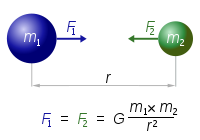
\includegraphics[width=3cm]{200px-NewtonsLawOfUniversalGravitation.png}
			\end{figure}
	\end{description}

\end{frame}
%\begin{frame}{Traditional View}
%
%	\begin{itemize}
%		\item Universal generalization, true for everything
%		\item Doesn't depends on the meanings of the constituent
%		\item It cannot be otherwise.
%	\end{itemize}
%\end{frame}

\begin{frame}{More precisely}
$\rightarrow$ Universal generalization

\vfill
The laws are ``laws of nature'', they apply on everything in the worlds, even if in probabilistic terms.

\end{frame}
\begin{frame}{More precisely}
$\rightarrow$ Doesn't depends on the meanings of the constituent

\vfill
It's always true given the empirical fact as the laws contains the empirical facts.
\end{frame}

\begin{frame}{More precisely}
$\rightarrow$ It cannot be otherwise

\vfill
Something that does not follow the laws cannot exist, or the theory is false and the laws should be changed.
\end{frame}

\begin{frame}{Semantic View}
	The theories becomes more like a definition than a set of laws:
	\vfill
	\begin{quote}
		A Newtonian mechanical system=[df] a system of objects which behave according to Newton's three laws of motion and the law of universal gravitation.\\
		Beatty (1980)
	\end{quote}
\end{frame}


\begin{frame}{Evolutionary Biology}
	Hardy Weinberg Equilibrium
	\begin{equation}
		p^2 + 2pq + q^2 = 1
		\label{eq:hw}
	\end{equation}
	with $p$ the freq. of allele A and $q$ the freq. of allele a in a pop with the phenotypes AA,Aa,aa
\end{frame}

\begin{frame}{Mendel's Law}
	This Hardy-Weinberg is a generalisation of the well known law of Mendel:
			\begin{figure}
				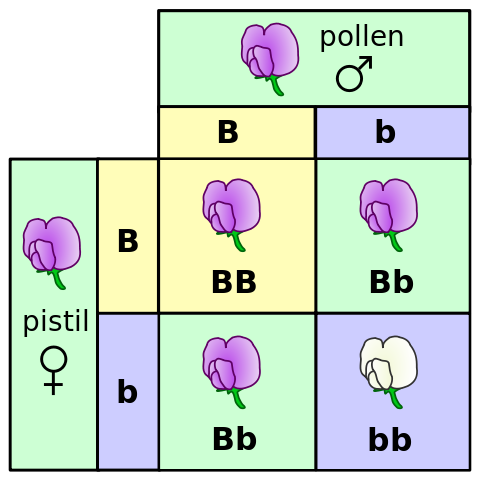
\includegraphics[width=3cm]{480px-Punnett_square_mendel_flowers.png}
			\end{figure}
	
\end{frame}
\begin{frame}
	\begin{center}
		Mendel + Hw Equilibrium
	\end{center}
	
	a neutral model that allow biologists, as Newton's law helps physicists, to see when systems move from this equilibrium and to point action of evolutionary strength such as Natural Selection, genetic drift\ldots 
\end{frame}

\begin{frame}{Problems}
	\begin{alertblock}
		{But is this Mendel law  a ``law''?}
	\end{alertblock}

	For the author, Mendel's law is not
	\begin{quote}
		an approximation of any physically necessary regularity.\\
		Beatty~(1980, p.~409)
	\end{quote}
	$\rightarrow$ It's a produce of the Natural Evolution.
\end{frame}


\begin{frame}{No Absolute Phenomena}
	Another way to see it, as reports Delbrück, is that :
	\begin{quote}
		[\ldots] there are no ``absolute phenomena'' in biology. Everything is time bound and space bound. \\
		Delbrück~(1952)
	\end{quote}
\end{frame}


\begin{frame}
	Mendel's law and HW equilibrium could be empirically true or not as under the semantic view :
	\vfill
	\begin{quote}
		[\ldots]	a theory is just the specification of a kind of system--more a definition than an empirical claim. \\
		Beatty (1980)
	\end{quote}

	
\end{frame}

\begin{frame}
	More precisely, theories are set of models that are true depending on a given meaning of the elements constitutive of those models.

	\begin{columns}
		\column{0.4\textwidth}
		\begin{figure}
			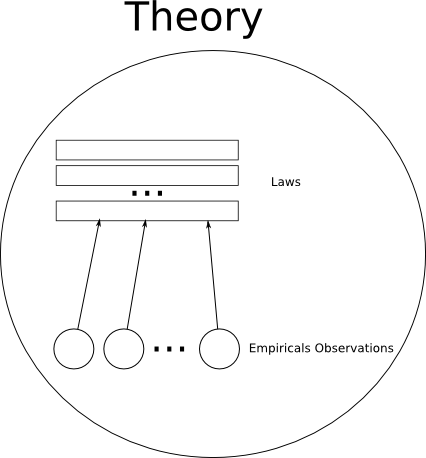
\includegraphics[height=3cm]{tradView.png}
			\caption{The Traditional View of Theories}
		\end{figure}

		\column{0.6\textwidth}
		\begin{figure}
			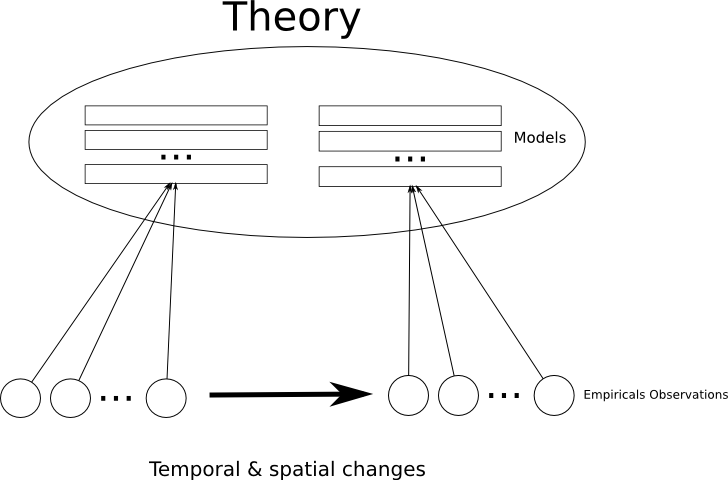
\includegraphics[height=3cm]{semView.png}
			\caption{Semantic View of Theories}
		\end{figure}
	\end{columns}
\end{frame}


\begin{frame}{The Semantic View of Theories}
	For Beatty:
	\begin{quote}
		The semantic view better accommodates the fact that evolutionary theory is bound to change as a result of the evolutionary process itself.\\
		Beatty (1980)
	\end{quote}
\end{frame}

\end{document}

